The same process as described in \autoref{sec:BeadsResults} can be repeated for other dataset, and the all the beads diameter and velocity can be estimated. This leads us to the true potential of IFC sensors in biological studies: Big Data. Big Data harnesses the power of numerical computations to efficiently extract relevant informations from enormous datasets. It could be imagined that a team of biologists collect the impedance data of millions of cells and particles using the portable device described in this memoir, and extract the important informations of these cells using Machine Learning, and high-end signal processing. \par

As a small-scale example, 7 datasets similar to the one obtained in \autoref{sec:BeadsResults} were collected and passed into the peak detection and classification algorithm. 2238 beads were detected and their magnitude, diameters, and velocity in the channels were calculated. \autoref{fig:BigDataMagnitudes}, \autoref{fig:BigDataDiameters}, and \autoref{fig:BigDataVelocity} show the distribution of these parameters. It is possible to see that the beads of sizes below 50 $\mu$m were not detected, simply because the impedance-sensing system lacks sensibility to detect such small impedance variations. The discrete distribution for the velocities should also be noted, which is a direct result of the lack of sampling points to characterize some of the faster velocities, as explained before in \autoref{sec:BeadsResults}. 
\begin{figure}[h]
\centering
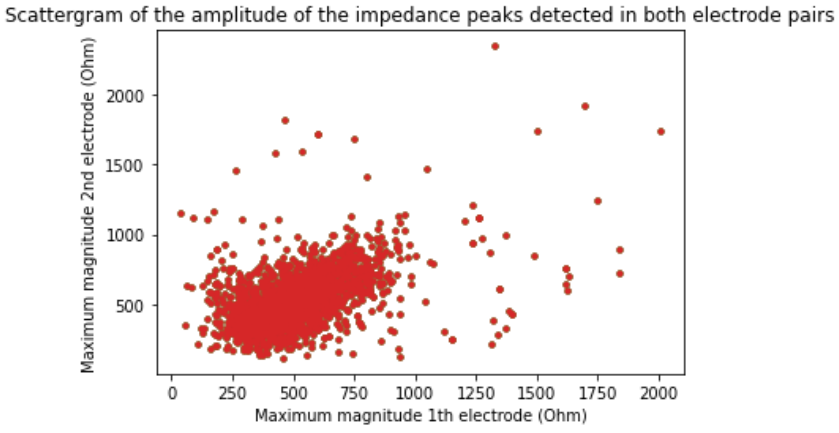
\includegraphics[width=0.99\linewidth]{BigDataMagnitudes}
\caption{Scattergram of the impedance magnitude measured by both electrode pair for the 2380 detected microbeads of sizes between 10 $\mu$m and 90 $\mu$m.}
\label{fig:BigDataMagnitudes}
\end{figure}

\begin{figure}[h]
\centering
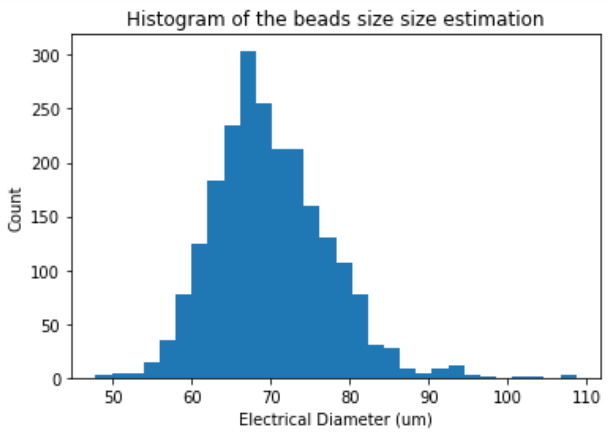
\includegraphics[width=0.7\linewidth]{BigDataDiameters}
\caption{Histogram of the estimated diameters of the 2380 detected microbeads of sizes between 10 $\mu$m and 90 $\mu$m.}
\label{fig:BigDataDiameters}
\end{figure}

\begin{figure}[h]
\centering
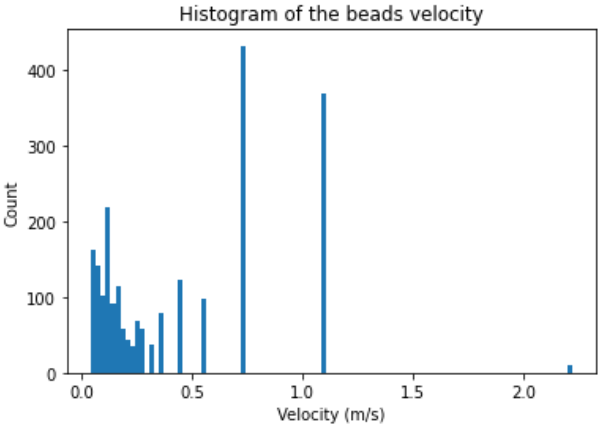
\includegraphics[width=0.7\linewidth]{BigDataVelocity}
\caption{Histogram of the particle velocity of the 2380 detected microbeads of sizes between 10 $\mu$m and 90 $\mu$m.}
\label{fig:BigDataVelocity}
\end{figure}